\chapter{Design}



%You should concentrate on the more important aspects of the design. It is essential that an overview is presented before going into detail. As well as describing the design adopted it must also explain what other designs were considered and why they were rejected.

%The design should describe what you expected to do, and might also explain areas that you had to revise after some investigation.

%Typically, for an object-oriented design, the discussion will focus on the choice of objects and classes and the allocation of methods to classes. The use made of reusable components should be described and their source referenced. Particularly important decisions concerning data structures usually affect the architecture of a system and so should be described here.

%How much material you include on detailed design and implementation will depend very much on the nature of the project. It should not be padded out. Think about the significant aspects of your system. For example, describe the design of the user interface if it is a critical aspect of your system, or provide detail about methods and data structures that are not trivial. Do not spend time on long lists of trivial items and repetitive descriptions. If in doubt about what is appropriate, speak to your supervisor.


\section{Overall Architecture}
The initial design for the robot is to produce a small wheeled vehicle with a platform for mounting the various systems.  These systems should be a central control unit, motor control and the various sensors.

\begin{figure}[h]
\centering
        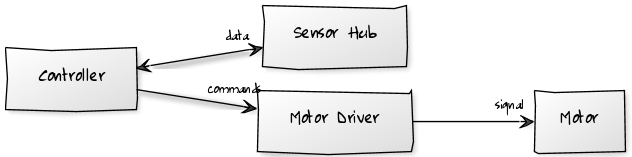
\includegraphics[width=4.0in] {Images/basic-uml.png}
        \caption{Basic system diagram}
        \label{Basic system diagram}
\end{figure}


\begin{figure}[h]
\centering
        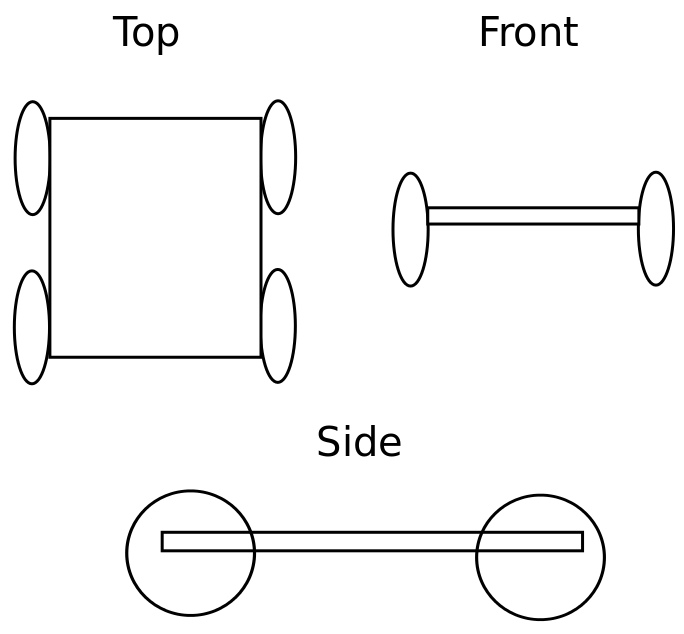
\includegraphics[width=2.0in] {Images/initial-design.png}
        \caption{Initial design}
        \label{Initial design}
\end{figure}

The central control unit will be a microcontroller for ease of interfacing directly with hardware as well as keeping power consumption down.  Keeping power consumption to a minimum is important so that the robot can be active for a longer period of time without needing to be recharged.  This controller will interface with both a motor control system and the various sensors required to detect objects in the environment local to the robot.

\section{Justifications}
The various components that the project will need to come together into a finished product have many options.
\subsection{Materials}
I considered several materials for the robot chassis to be built of.
\begin{itemize}
\item Wood
\\This would be the easiest material to make the chassis from as it is very cheap, easy to cut into the intended shape and easy to mount components on with either adhesive, nails or screws.  Also the fact that it does not conduct electricity will help when mounting circuit boards to it.

\item Plastic
\\The lightest option.  Good due to its low weight but may not be as strong as wood or a metal option and could bend or snap under the load of heavier components such as motors or a large power source.  It can be more expensive than wood to aquire.  There is a higher difficulty in cutting it into the desired shapes.  It is also non-conductive, again useful to mount electronic components to.  Plastic can hold a static

\item Steel
\\A stronger material that can withstand a much heavier load, but is itself rather heavy compared to wood or plastic.  This extra base weight before adding anything else will put more strain onto the motors used to drive the robot and may even need to use more powerfull motors because of this extra weight.  It is a very conductive material which means that a non-conductive mounting platform will also be needed to mount electronic components as to avoid damaging them.

\item Aluminium
\\A much lighter metal than steel, but still much heavier than wood or plastic or the same thickness.  It can also withstand heavier loads than wood or plastic but it also much more difficult to cut.  Again aluminium is a very conductive material meaning that a non-conductive mounting platform will be needed.  It can also be used as a heat sink for the components that can get very hot such as the motor drivers or the motors themselves.  A heatsink is a material attached to something that gets very hot and conducts that heat.  It generaly has a large surface area to disipate the heat into the cooler air around it, but it may also have a fan to blow/draw the hotter air away replacing it with air/gas with a lower temperature than that of the heatsink.

\end{itemize}

Aluminium seems to be the best all round choice being strong but not as heavy as steel.  It can act as a heat sink if the motors are mounted directly to it.  It is also not very expensive to buy in small amounts.
\\In addition to the aluminium base I have decided to use plastic for mounting components to the base as it is light, inexpensive and non conductive which is suitable for electronic components.

\subsection{Actuators}
Actuators are motors used for controlling movement of a system.
\begin{itemize}
\item Servo
\\Typical servos are a motor and a gearbox with a potentiometer, a voltage divder in this case used to determine how far a motor has turned, for feedback.  These motors are great for controling such things as the direction of sensors or moving very light devices.  Servos are low voltage, typically 4.8 - 6 volts, and as such do not have much strength, they are typicaly not good for driving larger equipment.  Also most servos only turn up to 180 degrees or 360 degrees.  In normal operation they do not turn continuously but can be modified to do so at the cost of losing the feedback of how far the motor has turned.
\begin{figure}[h]
\centering
        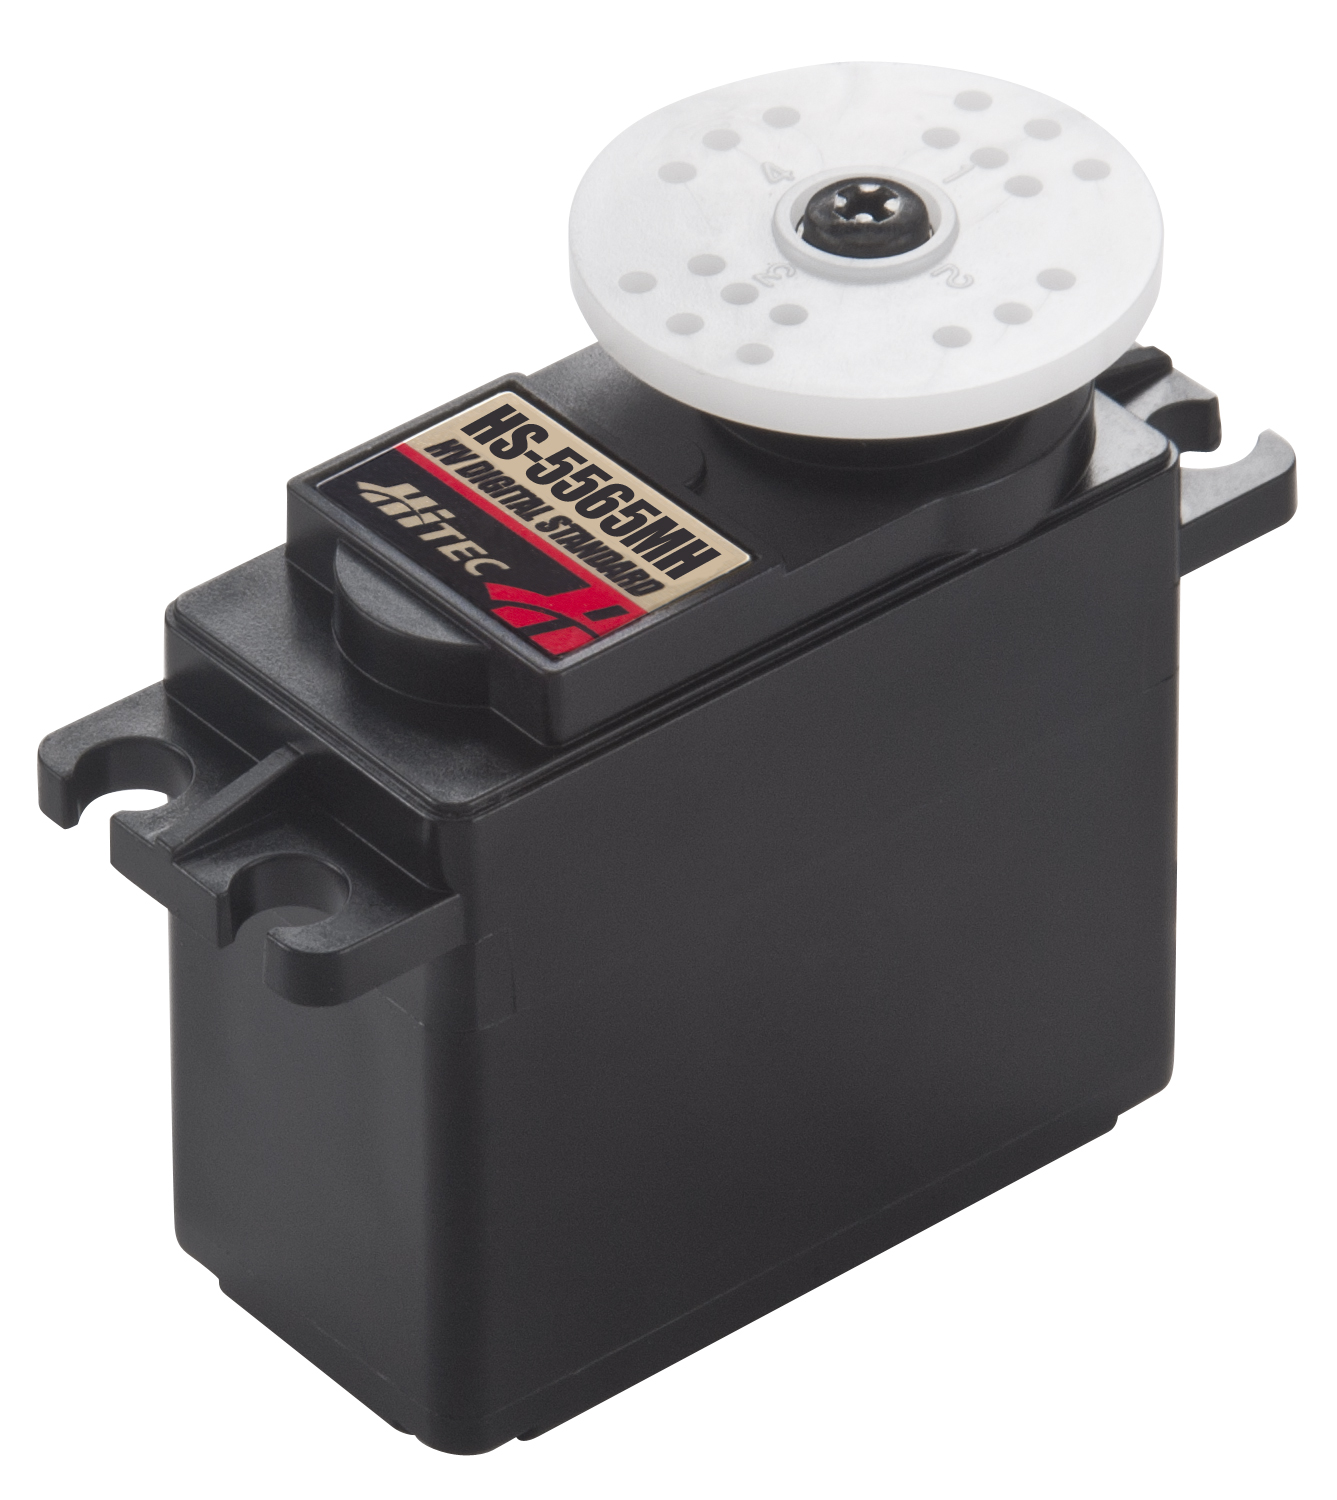
\includegraphics[width=1.5in] {Images/servo.jpg}
        \caption{Servo Motor - robotshop.com}
        \label{Servo Motor}
\end{figure}

\item DC Motor
\\Direct current motor has a very simple operation.  Apply current to one side of the motor to make it turn, reverse the direction of the current to reverse the direction the motor turns.  Changing the speed of these motors is simple, either change the voltage, keeping it within the devices tolerances, or turn the current supplied to the motor on and off at high speed where how quickly it is alternated determines the speed of the motor.  Typicaly these motors are attached to a gearbox to gain more torque to drive much higher loads.  Optical rotary encoders can be used to determine how much the motors have turned and how fast.  These encoders use a light based sensor to detect when the light changes in front of it, this can be used with a disc that has black and white lines on it.  The change in color is detected, this along with how many times it changes and with what frequency this happens can determine the amount a wheel has turned and how fast it has done so.
\begin{figure}[h]
\centering
        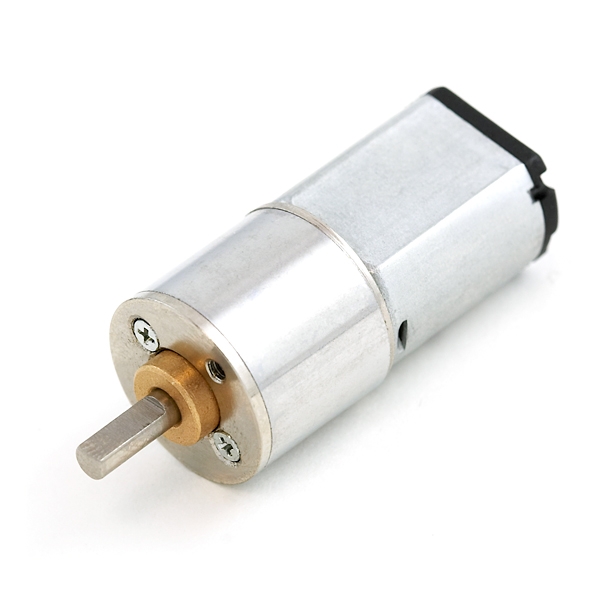
\includegraphics[width=2.0in] {Images/dc-motor.jpg}
        \caption{DC Motor - sparkfun.com - CC BY-NC-SA 3.0}
        \label{DC Motor}
\end{figure}
\item Steppers
\\Stepper motors use an internal gear and a ring of magnets.  These magnets pull the gear into position, powering the magnets in sequence which will turn the motor.  Each part of this cycle is called a step.  This means that a single step is a know amount of rotation.  Using this type of motor ensures that you can accuratly turn whatever is attached to the motor shaft a known amount without any additional measuring equipment, although it may be used to verify that it has in fact moved the amount expected
\begin{figure}[h]
\centering
\begin{subfigure}
	\centering
        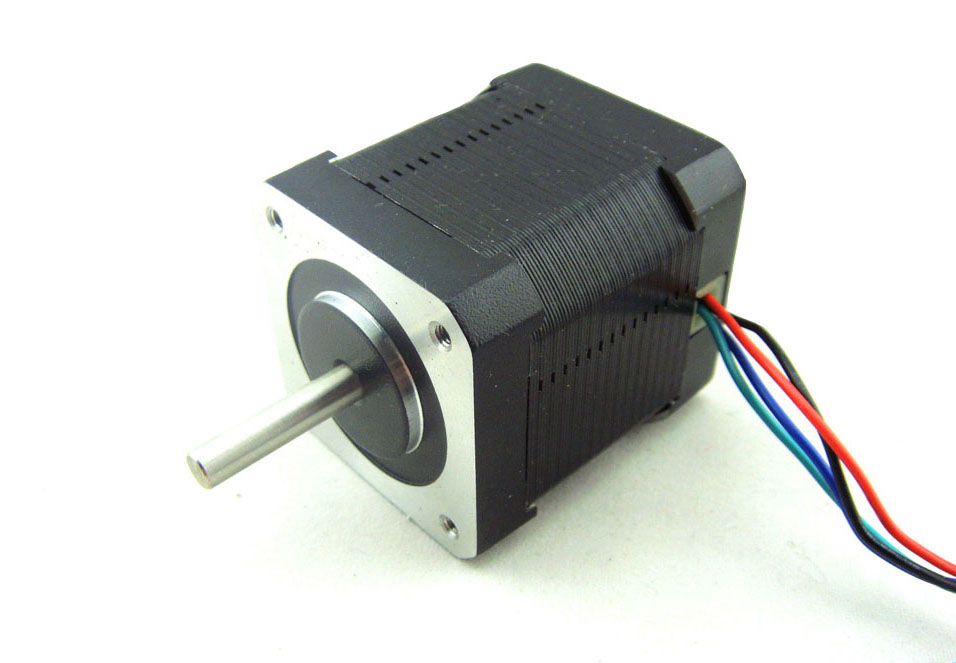
\includegraphics[width=2.0in] {Images/stepper.jpg}
        \caption{Stepper Motor - stepperonline.com}
        \label{Stepper Motor}
\end{subfigure}
\begin{subfigure}
        \centering
        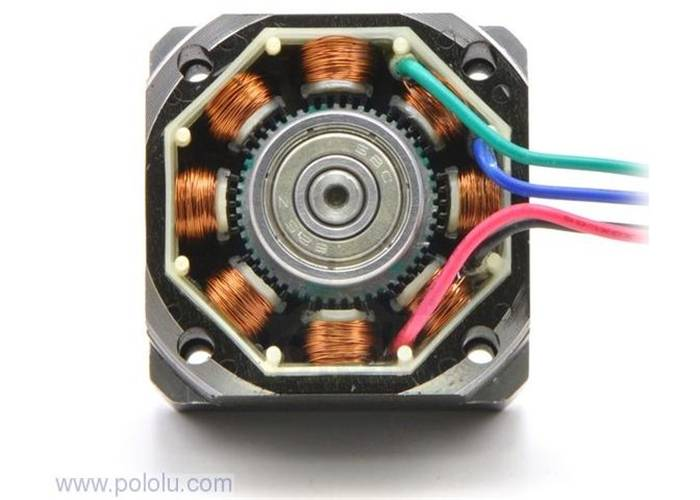
\includegraphics[width=2.0in] {Images/stepper-internal.jpg}
        \caption{Stepper Motor Internal- robotgear.com.au}
        \label{Stepper Motor Internal}
\end{subfigure}
\end{figure}
\end{itemize}

I have chosen to use stepper motors due to the ability to control the amount and speed of rotation with more accuracy than the alternatives.  Stepper motors do come in high torque version which may be needed for this project as the chassis is made of metal which is a much hevaier material.  A stepper motor could be using with a chassis of any of the materials mentioned, it may struggle with steel depending on how thick of a piece is used.  DC motos could also be used with all materials if in conjunction with a gearbox, but the additional system needed to measure and control the exact rotation of the wheels using this method puts me off of the idea.  Greater power but less accurate control.

\subsection{Sensors}

\begin{itemize}
\item LDR
\\An LDR is a light dependant resistor.  A small resistor that changes its resistance depending on how much light it is exposed to.  This could be used to detect if the robot is very close to bumping into an object and avoid it as the object got closer and possibly cast a shadow onto the sensor reducing the amount of light the resistor can detect, kind of like a physical bump skirt which activates when something touches it.
\begin{figure}[h]
\centering
        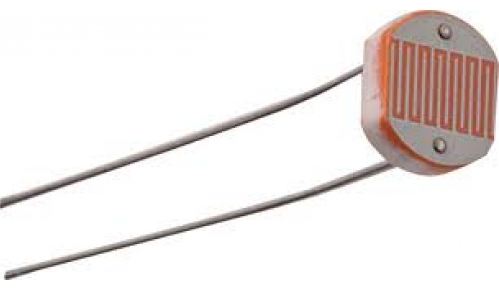
\includegraphics[width=2.0in] {Images/ldr.jpg}
        \caption{Light Dependant Resistor - robotics.org.za}
        \label{Light Dependant Resistor}
\end{figure}

\item Camera
\\A camera could be used to detect objects in front of it using various image processing techniques.  This method is good because it can potentialy map a relatively large area in a single image.  On the other hand it requires more processing to do, which can be slow and result in coliding into an object or being stuck in a tight space before the system has finished processing data from the camera.  I could use a more powerful processor to overcome this but it adds complexity, cost and power consumption.
\begin{figure}[h]
\centering
        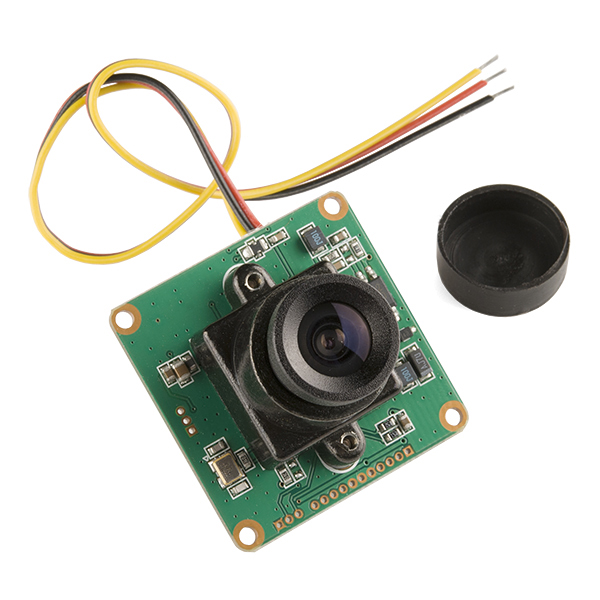
\includegraphics[width=2.0in] {Images/camera.jpg}
        \caption{Camera Module - sparkfun.com - CC BY-NC-SA 3.0}
        \label{Camera Module}
\end{figure}

\item Infrared
\\Used to detect distance from an object.  An emiter and a receiver pair linked to work like the light dependent resistor but using infrared instead of normal visible light.  Depending on the intensity of infrared picked up by the reciever it can be used to determine the distance from the source of the reflection.  Ambient infrared can effect readings as there is infrared radiation emitted from the sun and is everywhere.  This extra radiation other than the amount emitted by the sensor is un-needed and unwanted and as such if it arrives at the reciever the readings will be inaccurate from those expected.
\begin{figure}[h]
\centering
        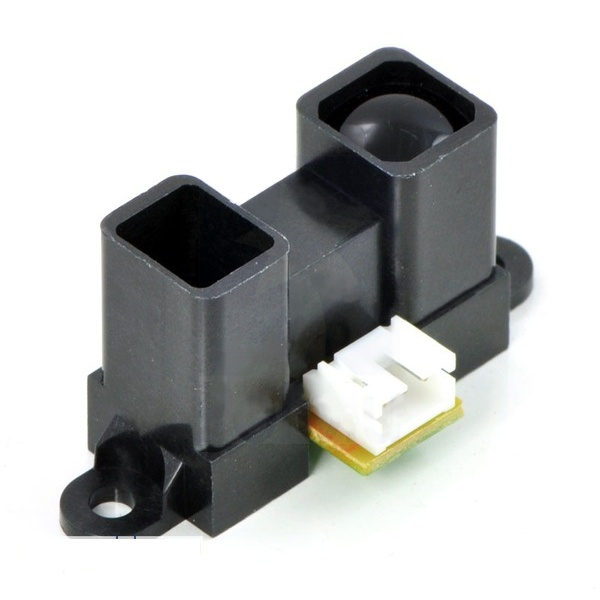
\includegraphics[width=2.0in] {Images/ir.jpg}
        \caption{Infrared Sensor - coolcomponents.co.uk}
        \label{Infrared Sensor}
\end{figure}

\item Sonar
\\Again an emitter style approach.  It emits an ultrasonic wave to bounce off of whatever surface is in front of it.  The time taken from emitting the wave until recieving the wave determines how far away the object is.  This method comes with its drawbacks.  Due to how sound waves behave when they interact with the environment by bouncing off of it.  If the surface is angled or curved the sound can bounce away from the reciever, either not reaching it at all giving the possible false reading that there is nothing in front of it, or it could bounce off of multiple surfaces back to the reciever giving a false reading that an object is there but further away due to the sound taking longer than it should have to reach the reciever.
\begin{figure}[h]
\centering
        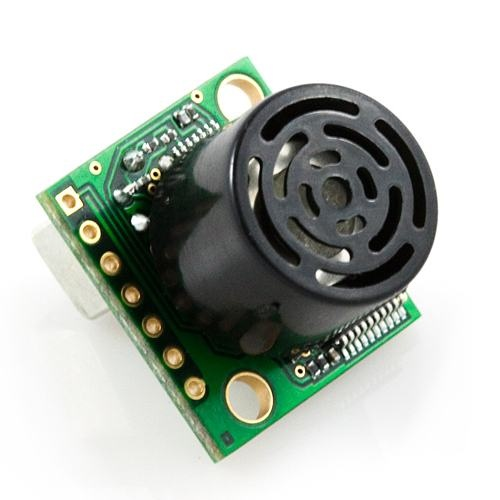
\includegraphics[width=2.0in] {Images/sonar.jpg}
        \caption{Ultrasonic Sensor - coolcomponents.co.uk}
        \label{Ultrasonic Sensor}
\end{figure}

\end{itemize}
A combination of both sonar and infra red logicaly seems like a good idea.  One can compensate for the others weaknesses.  Use the sonar to compensate for ambiant infra red and the infra red can be used to compensate for sonar bouncing around the environment.  Hopefully this will reduce the number of false readings produced.
\subsection{Control}
The robot will need a controler, that connects the software to all the hardware.
\begin{itemize}
\item PIC
\\Peripheral Interface Controller.  Very low cost microcontroller with a small easy to learn instruction set and support serial communication/re-programming.  They also come in a DIL package (dual in-line) making them easy to incorporate into through-hole printed circuit boards as the legs of the chips can fit through these holes and be soldered (held in place with a low melting point conductive metal alloy.) into place.
\begin{figure}[h]
\centering
        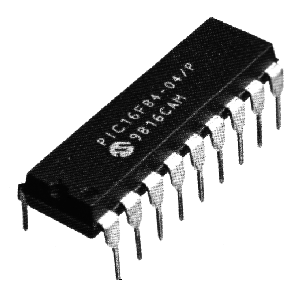
\includegraphics[width=2.0in] {Images/pic-chip.png}
        \caption{PIC - circuitstoday.com}
        \label{PIC}
\end{figure}

\item Arduino
\\An open source hardware board that is cheap but not as cheap as a PIC.  These are very popular among hobbyists due to them being very easy to use and having a vast collection of community written libraries to interface with all different types of hardware.
\\Arduino uses C or C++ programming language for development.
\begin{figure}[h]
\centering
        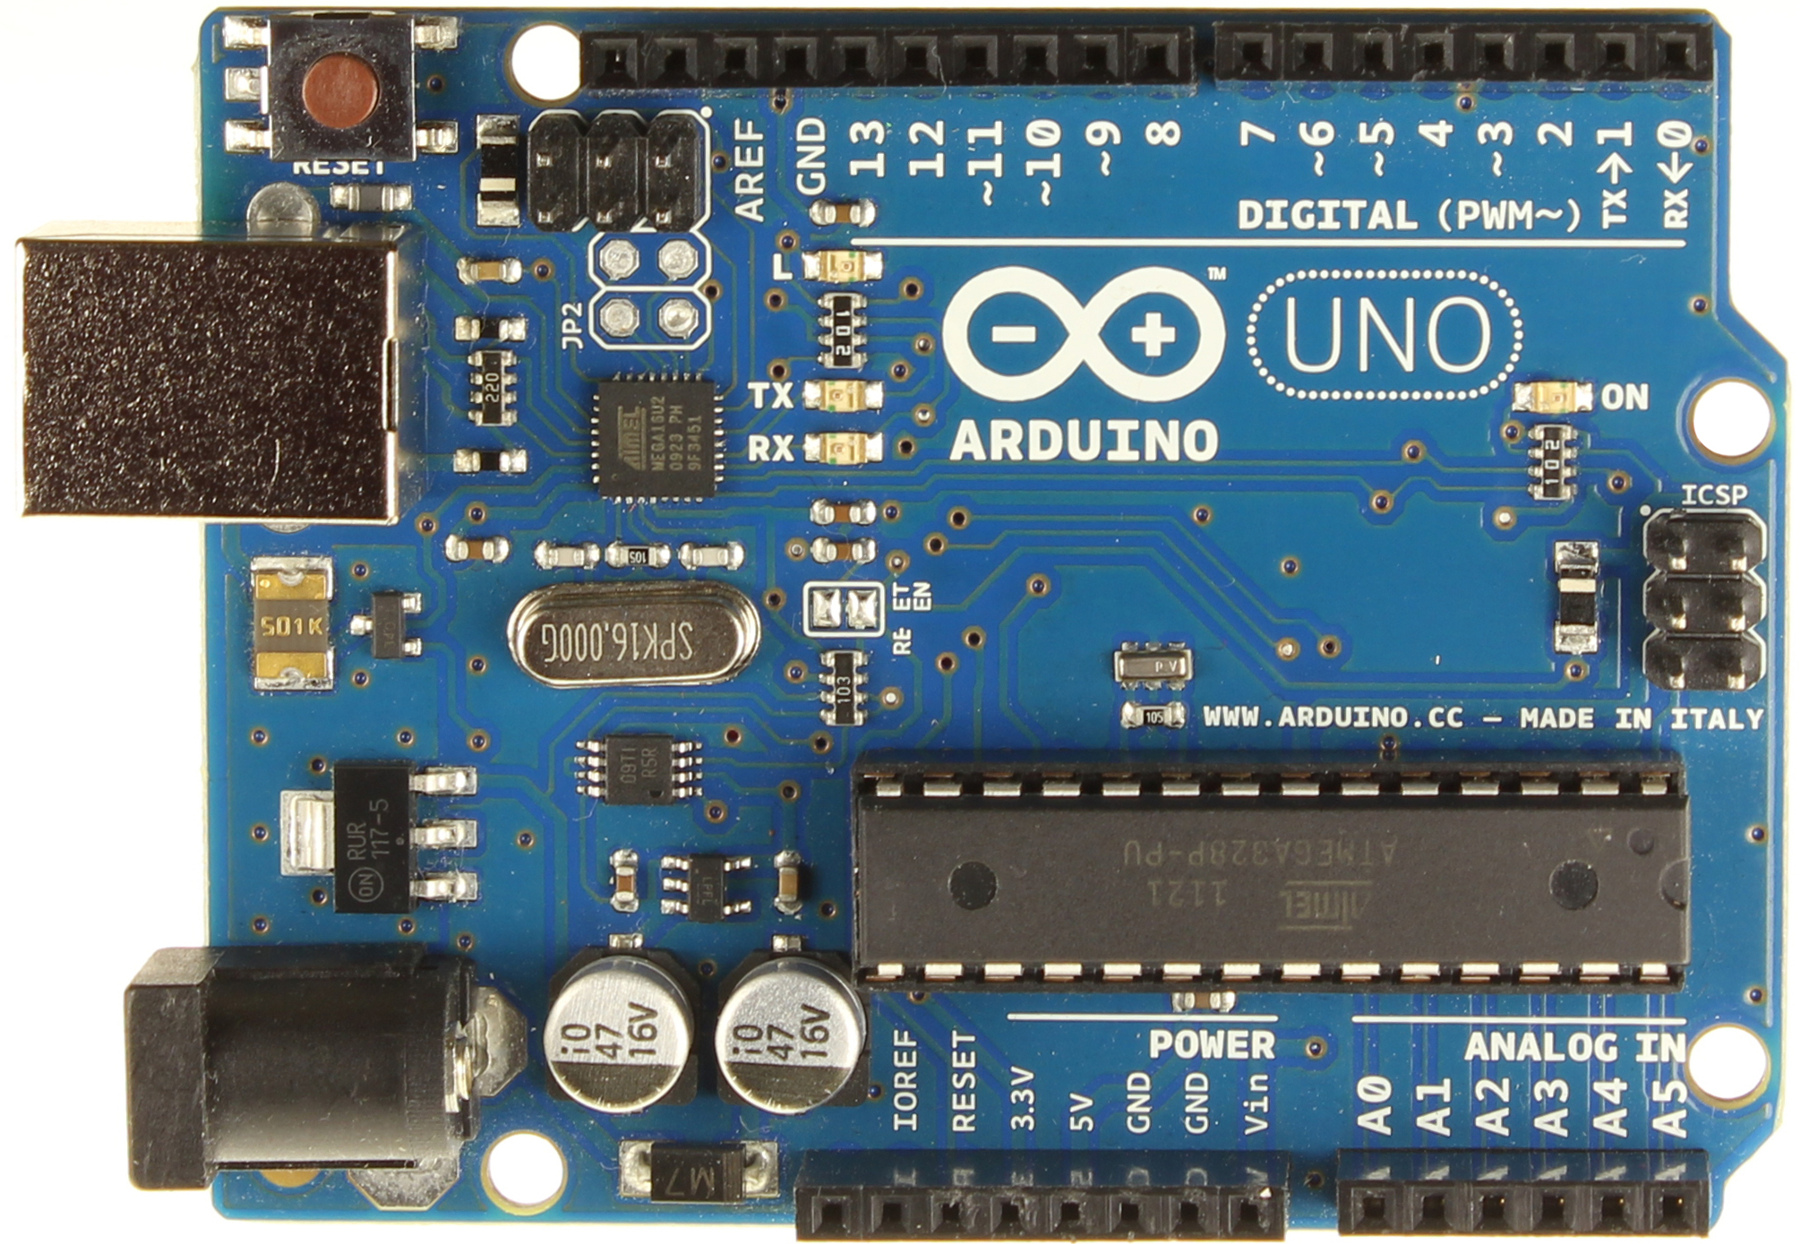
\includegraphics[width=2.0in] {Images/arduinouno-r3.jpg}
        \caption{Arduino arduino.cc}
        \label{Arduino}
\end{figure}

\item Netduino
\\This is also an open source electronics prototyping platform but instead of being based on C and C++ it is based on the .Net Micro Framework which is Microsoft's version of an embedded framework.
\\These boards cost more than the Arduino and PIC, and have much less community support.
\begin{figure}[h]
\centering
        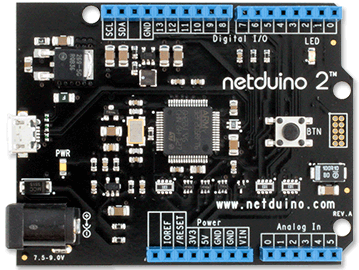
\includegraphics[width=2.0in] {Images/netduino.png}
        \caption{Netduino - netduino.com}
        \label{Netduino}
\end{figure}

\item Motherboard
\\A small motherboard that can be found in a home computer or a netbook/laptop.  These have the widest variety of applications.  It can support most operating systems and programming languages but come at the hefty price of power consumption.  Compared to microcontrollers, a full motherboard draws a very large amount of power to run compared to the comsumption of a microcontroller.  Also they take far longer to power on due to running an operating system, unlike microcontrollers that have the code compiled down and run directly on the hardware itself.
\\The cost of such boards is also very high as they are far more complex pieces of electronics.
\begin{figure}[h]
\centering
        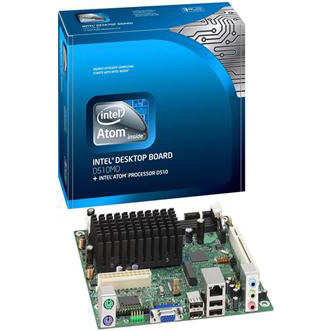
\includegraphics[width=2.0in] {Images/atom.jpg}
        \caption{Atom Motherboard - intel.co.uk}
        \label{Atom Motherboard}
\end{figure}
\item Raspberry Pi
\\The Raspberry Pi is a credit card sized computer that is an embedded platform for Linux and various other operating systems.  It is very cheap and runs much faster than most microcontrollers.  It does also have the downside of long startup times due to running a full desktop style operating system on such a compact board.  Unlike normal motherboards this little board has some GPIO (general purpose input output) pins for interacting directly with various pieces of hardware like the microcontrollers do.
\begin{figure}[h]
\centering
        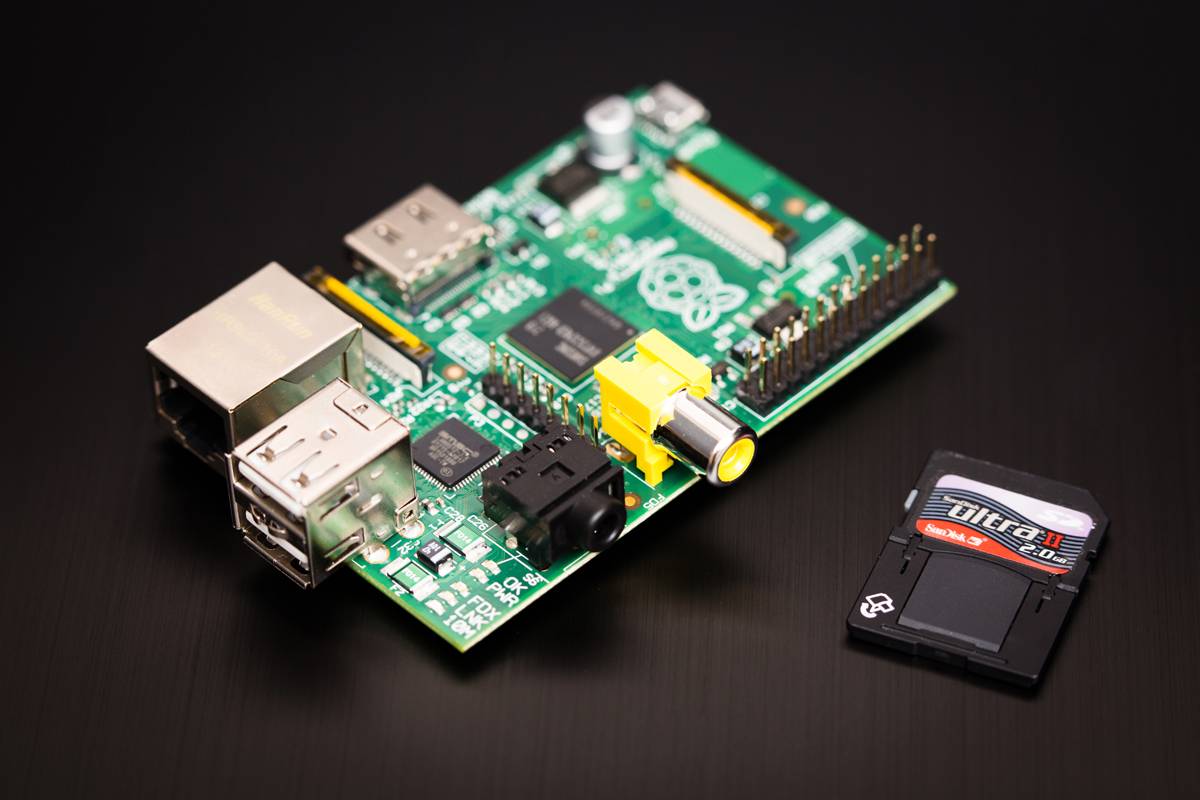
\includegraphics[width=2.0in] {Images/rpi.jpeg}
        \caption{Raspberry Pi - raspberrypi.org}
        \label{Raspberry Pi}
\end{figure}

\end{itemize}

\subsection{Power Source}
As this robot is intended to move around freely, unhindered by power and data cables, the powersource cannot be supplied by a wall power outlet, it has to be self contained.  This means it will have to be a battery.  The battery will have to be several cells or a single high output cell due to the size of motors intended.
\\I will need as many Amp hours as possible for longer runtimes.  This could be achieved with several cells linked together in series (end to end) to increase voltage and/or link more together in parrallel (side by side) to increase amp hours (runtime).
\begin{itemize}
\item Lithium Polymer
\\LiPo batteries come in up to 11.2 volt packages, which is not quite high enough for some higher voltage motors which I may be using such as the high end steppers.  These batteries are much lighter than some other alternatives and are common in embedded devices.
\begin{figure}[h]
\centering
        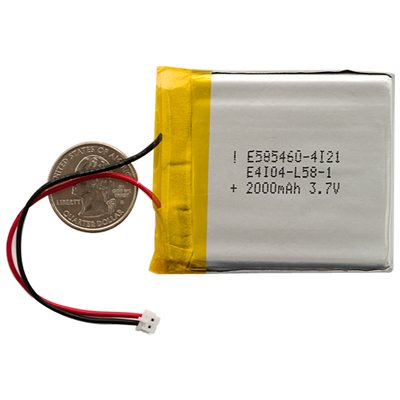
\includegraphics[width=2.0in] {Images/lipo-front.jpg}
        \caption{Lithium Polymer Battery - robotshop.com}
        \label{Lithium Polymer Battery}
\end{figure}

\item Lead Acid
\\A lead acid battery is a choice with a high output.  A single battery can output 12 volts and can be found in high amp hour packages such as 1 - 40amp hours compared to the lithium alternatives which are around 0.1 - 6 amp hours.  Due to needed a high power motor for the chassis already, a higher weight battery is not too much of an issue and provides the benefit of the higher power output.
\end{itemize}
\begin{figure}[h]
\centering
        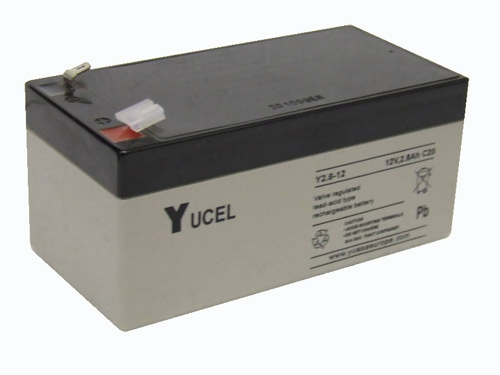
\includegraphics[width=2.0in] {Images/lead-acid.jpg}
        \caption{Lead Acid Battery - kestrelelectricalsupplies.co.uk}
        \label{Lead Acid Battery}
\end{figure}

\section{Feedback Interface}
While operating the robot, if there is any unexpected behaviour it would be nice to have some form of interface to see what the robot thinks the environment looks like.  There cannot be any cables trailing from the robot to a laptop so a wireless solution would be good.
\\All that is needed is a small microcontroller, a wireless module and a display.
An Arduino Fio is a good fit as it is small, low powered, has both lithium polymer battery socket and an xbee wireless module socket built in.
\\A small LCD (liquid crystal display) can be connected to the Arduino to display information it recieves.

